\newcommand{\missing}[1]{{\color{red}\bfseries [TODO]}}

\newcommand{\egg}{\texorpdfstring{\MakeLowercase{\texttt{egg}}}{\texttt{egg}}\xspace}
\newcommand{\Egg}{\texorpdfstring{\MakeLowercase{\texttt{egg}}}{\texttt{egg}}\xspace}
\newcommand{\egraphs}{\mbox{e-graphs}\xspace}
\newcommand{\egraph}{\mbox{e-graph}\xspace}
\newcommand{\Egraph}{\mbox{E-graph}\xspace}
\newcommand{\Egraphs}{\mbox{E-graphs}\xspace}
\newcommand{\eclass}{\mbox{e-class}\xspace}
\newcommand{\Eclass}{\mbox{E-class}\xspace}
\newcommand{\enode}{\mbox{e-node}\xspace}
\newcommand{\eclasses}{\mbox{e-classes}\xspace}
\newcommand{\enodes}{\mbox{e-nodes}\xspace}
\newcommand{\Enodes}{\mbox{E-nodes}\xspace}
% \newcommand{\regraph}{Regraph\xspace}
% \newcommand{\Regraph}{Regraph\xspace}
\newcommand{\sz}{Szalinski\xspace}
\newcommand{\find}{\texttt{find}\xspace}

\newcommand{\equivid}{\equiv_{\sf id}}
\newcommand{\equivnode}{\equiv_{\sf node}}
\newcommand{\equivterm}{\equiv_{\sf term}}

\newcommand{\congrinv}{$\mathcal{I}_c$\xspace}

\newcommand{\egglogo}[1][]{\protect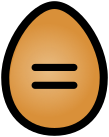
\includegraphics[height=1em, #1]{egg.png} }
\newcommand{\eggurl}{\url{https://github.com/mwillsey/egg}}

% TODOs
% https://tex.stackexchange.com/questions/9796/how-to-add-todo-notes

\newcommand{\eggtodo}[1]{\textcolor{Red}{\textbf{[CITE: #1]}}}

\newcommand{\defTodo}[2]{%
  \expandafter\newcommand\csname #1\endcsname[1]{%
    \todo[linecolor=#2,backgroundcolor=#2!25,bordercolor=#2,inline,size=\tiny]{\textbf{#1}: ##1}}}

\newcommand{\defTODO}[2]{%
  \expandafter\newcommand\csname #1\endcsname[1]{%
    \todo[linecolor=#2,backgroundcolor=#2!25,bordercolor=#2,inline,size=\tiny,caption={\textbf{(#1 LONG TODO)}}]{##1}}}

\newcommand{\LeoColor}{Goldenrod}
\newcommand{\MaxColor}{RoyalBlue}
\newcommand{\RemyColor}{Red}
\newcommand{\OliverColor}{OliveGreen}
\newcommand{\ChandraColor}{Magenta}
\newcommand{\PavelColor}{Cerulean}
\newcommand{\ZachColor}{Plum}
\newcommand{\BenColor}{Orchid}
\newcommand{\JamesColor}{Salmon}

\defTodo{Leo}{\LeoColor}
\defTodo{Max}{\MaxColor}
\defTodo{Remy}{\RemyColor}
\defTodo{Oliver}{\OliverColor}
\defTodo{Chandra}{\ChandraColor}
\defTodo{Pavel}{\PavelColor}
\defTodo{Zach}{\ZachColor}
\defTodo{Ben}{\BenColor}
\defTodo{James}{\JamesColor}

\defTODO{LEO}{\LeoColor}
\defTODO{MAX}{\MaxColor}
\defTODO{REMY}{\RemyColor}
\defTODO{OLIVER}{\OliverColor}
\defTODO{CHANDRA}{\ChandraColor}
\defTODO{PAVEL}{\PavelColor}
\defTODO{ZACH}{\ZachColor}
\defTODO{BEN}{\BenColor}
\defTODO{JAMES}{\JamesColor}

\newcommand{\CongrSpeedup}{\ensuremath{87.85\times}\xspace}
\newcommand{\TotalSpeedup}{\ensuremath{20.96\times}\xspace}
\newcommand{\RepairsR}{\ensuremath{0.98}\xspace}
\newcommand{\RepairsP}{3.6e-47\xspace}
\newcommand{\nEggTests}{32\xspace}
\newcommand{\nEggTimeouts}{8\xspace}


%%% Local Variables:
%%% TeX-master: "thesis"
%%% End:
